Before settling on attention as the signal to supervise, we surveyed how to read saliency out of a VLM at all. This appendix documents that exploratory study; it motivates the design choices of \Cref{sec:background} (mean aggregation over layers and heads; attention rather than gradients) and is not part of the main evaluation.

Saliency maps visualize the local importance of image regions for predicting a token. They are most commonly derived from the VLM's attention, though some methods also incorporate the prediction's gradients. We investigated raw attention, raw gradients, GradCAM~\citep{Selvaraju_2019}, and AGCAM~\citep{leem2024attention}, computing gradients from the backward pass of the token of interest (\Cref{fig:fourcats} compares all four). Map quality varied strongly with both the image and the prompt.

\textbf{Raw attention} was typically sparse. Sometimes it gave a very clear read on where the model looked (\Cref{fig:planes_attn}); other times it scattered seemingly at random onto background or image edges. Unlike gradient methods, attention placed high scores on only a few patch tokens (e.g., one or two patches near a cat's head), which covers small objects well but leaves large ones only partially highlighted.

\begin{figure}[t]
    \centering
    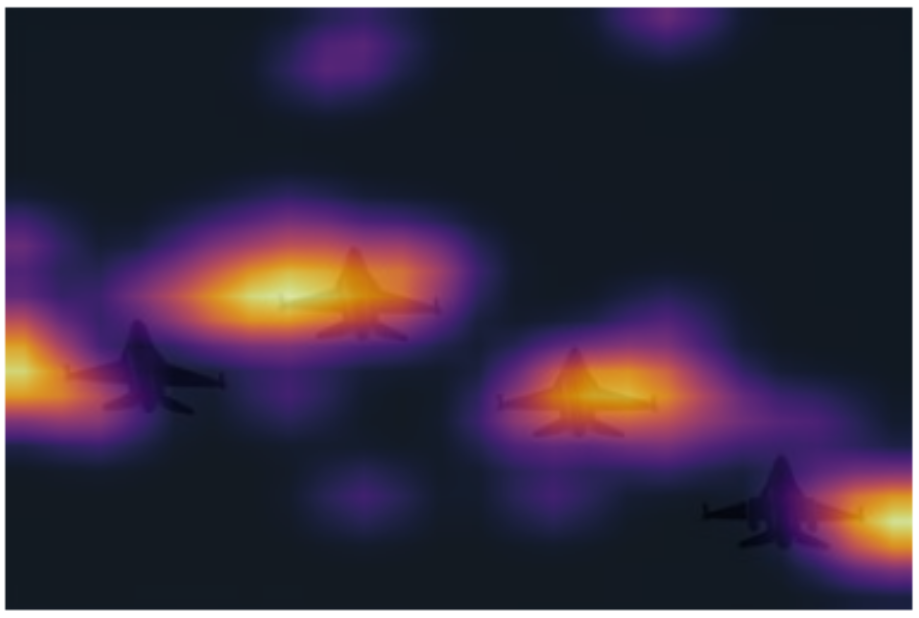
\includegraphics[width=0.8\linewidth]{figures/planes_attn.png}
    \caption{Attention saliency when the model is asked to count four planes.}
    \label{fig:planes_attn}
\end{figure}

\textbf{Raw gradients} behaved oppositely: broadly distributed, with high scores on many tokens. In useful cases two regimes appeared: either the gradients fully covered the region of interest, or they concentrated entirely on irrelevant areas, the inverse of the correct map. Our maps suggest, though do not confirm, that the first regime coincides with correct predictions and the second with incorrect ones. We also observed no visual correspondence between a layer's attention map and its gradient map.

\textbf{CAM variants} mix attention and gradients with simple transforms (e.g., ReLU). These were hit-or-miss: when they worked they produced maps that cleanly covered the objects of interest, but roughly a quarter of the time they were less interpretable than either ingredient. AGCAM (which additionally applies a sigmoid to the attention) produced the best maps when it worked but was less consistent than the more reliably interpretable GradCAM. We see room for a CAM variant tuned specifically to VLMs.

\textbf{Layers and heads.} Early-layer attention maps were far more interpretable than late-layer ones, where contextualized tokens attend less to the image. We saw strong evidence for localization heads~\citep{kang2025your} (a few heads do most of the looking and yield the cleanest maps), though the spatial-entropy heuristic for finding them was only mediocre.

\textbf{Aggregation and transforms.} Among aggregation rules, mean, max, and sum worked best, in that order; individual heads were complementary, each attending where others did not. Binarization and Gaussian smoothing both improved interpretability.

\begin{figure}[t]
    \centering
    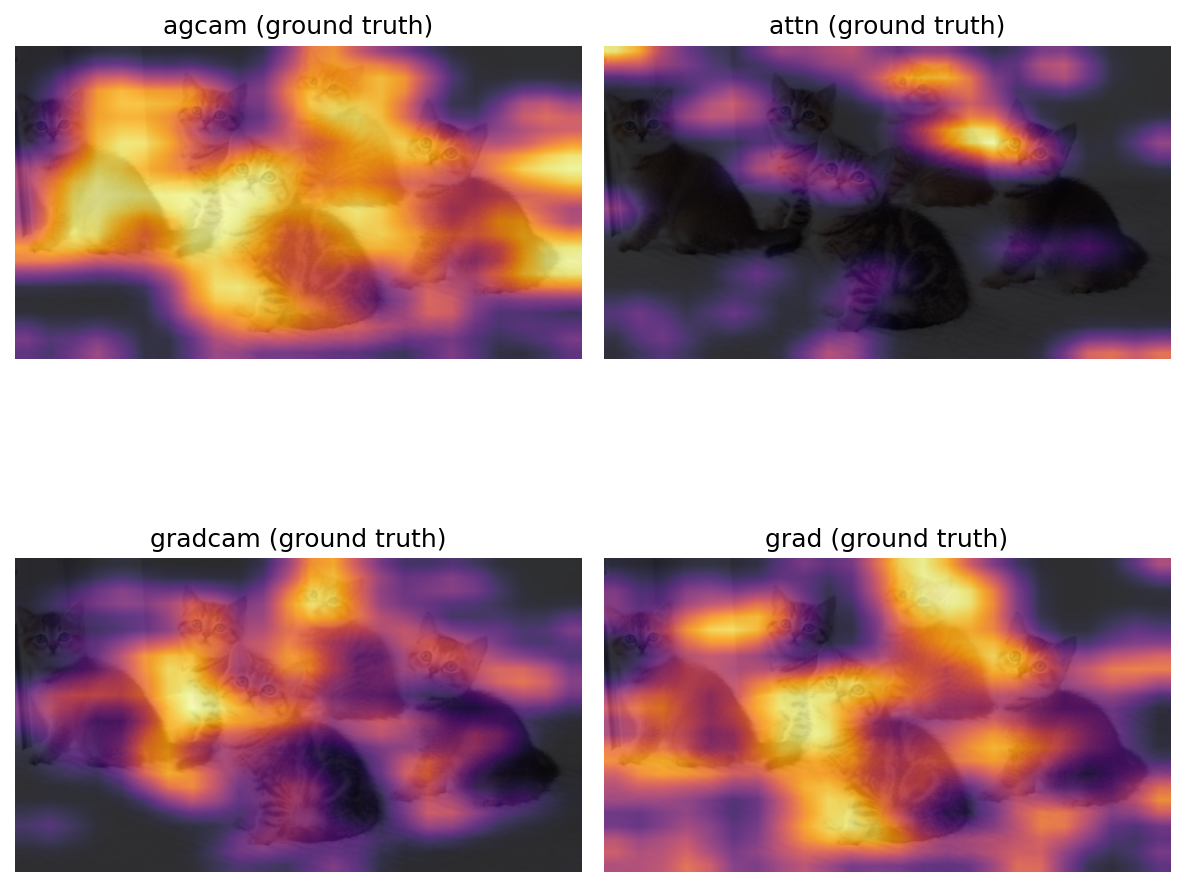
\includegraphics[width=0.8\linewidth]{figures/fourcats.png}
    \caption{The four attribution methods for the token ``four'' in the prompt \emph{``How many cats are in the image? There are four cats.''}}
    \label{fig:fourcats}
\end{figure}
